
    \tikzstyle{bagMain} = [text width = 3cm]
    
    \tikzstyle{bagMinor} = [text width = 3cm,
 		                    text = gray
 		                    ]

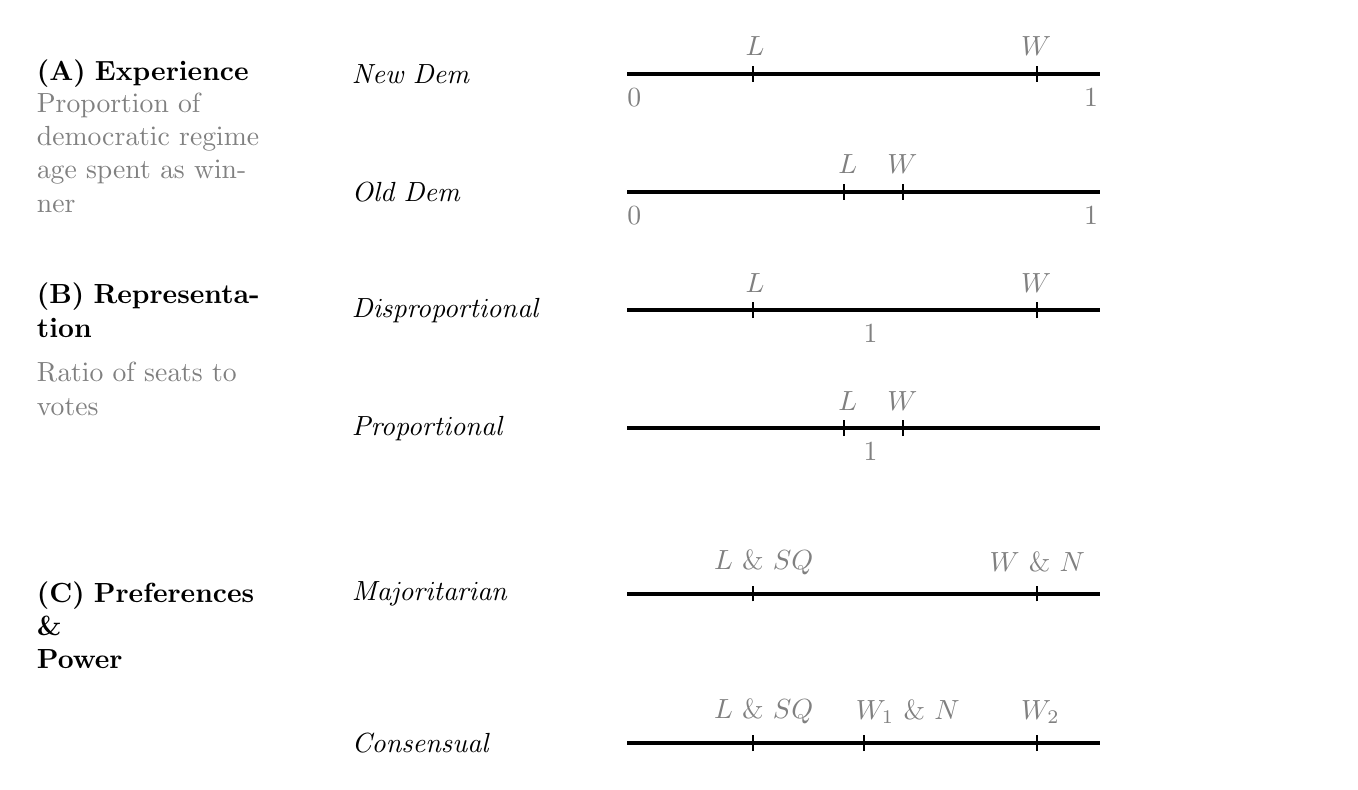
\begin{tikzpicture}


    %%% Gap Types
    % Experience %
    \node (E) at (-10, 5) [bagMain]{{\bf{(A) Experience}}};
    \node (Em) at (-10, 4) [bagMinor]{Proportion of democratic regime age spent as winner};
    
    \node (ND) at (-6, 5) [bagMain]{{\emph{New Dem}}};
    \node (OD) at (-6, 3.5) [bagMain]{{\emph{Old Dem}}};
    
    %%% Examples
    % New Dem
    \draw[line width = 0.5mm] (-4, 5) -- (2, 5);
    \node (N0) at (-2.5, 4.7) [bagMinor]{0};
    \node (N1) at (3.3, 4.7) [bagMinor]{1};
    
        % Losers 
        \draw[line width = 0.25mm] (-2.4, 4.9) -- (-2.4, 5.1);
        \node (NL) at (-1, 5.35) [bagMinor]{$L$};
    
        % Winners
        \draw[line width = 0.25mm] (1.2, 4.9) -- (1.2, 5.1);
        \node (NL) at (2.5, 5.35) [bagMinor]{$W$};
        
    % Old Dem
    \draw[line width = 0.5mm] (-4, 3.5) -- (2, 3.5);
    \node (N0) at (-2.5, 3.2) [bagMinor]{0};
    \node (N1) at (3.3, 3.2) [bagMinor]{1};
        
        % Losers 
        \draw[line width = 0.25mm] (-1.25, 3.4) -- (-1.25, 3.6);
        \node (NL) at (0.18, 3.85) [bagMinor]{$L$};
    
        % Winners
        \draw[line width = 0.25mm] (-0.5, 3.4) -- (-0.5, 3.6);
        \node (NL) at (0.8, 3.85) [bagMinor]{$W$};
        
        
    % Representation %
    \node (E) at (-10, 2) [bagMain]{{\bf{(B) Representation}}};
    \node (Em) at (-10, 1) [bagMinor]{Ratio of seats to votes};
    
    \node (ND) at (-6, 2) [bagMain]{{\emph{Disproportional}}};
    \node (OD) at (-6, 0.5) [bagMain]{{\emph{Proportional}}};
    
    %%% Examples
    % Disproportional 
    \draw[line width = 0.5mm] (-4, 2) -- (2, 2);
    \node (N1) at (0.5, 1.7) [bagMinor]{1};
    
        % Losers 
        \draw[line width = 0.25mm] (-2.4, 1.9) -- (-2.4, 2.1);
        \node (NL) at (-1, 2.35) [bagMinor]{$L$};
    
        % Winners
        \draw[line width = 0.25mm] (1.2, 1.9) -- (1.2, 2.1);
        \node (NL) at (2.5, 2.35) [bagMinor]{$W$};
        
    % Proportional
    \draw[line width = 0.5mm] (-4, 0.5) -- (2, 0.5);
    \node (N1) at (0.5, 0.2) [bagMinor]{1};
        
        % Losers 
        \draw[line width = 0.25mm] (-1.25, 0.4) -- (-1.25, 0.6);
        \node (NL) at (0.18, 0.85) [bagMinor]{$L$};
    
        % Winners
        \draw[line width = 0.25mm] (-0.5, 0.4) -- (-0.5, 0.6);
        \node (NL) at (0.8, 0.85) [bagMinor]{$W$};
        
    % Preferences & Power %
    \node (E) at (-10, -2) [bagMain]{{\bf{(C) Preferences \\ \& \\ Power }}};
    
    \node (ND) at (-6, -1.6) [bagMain]{{\emph{Majoritarian}}};
    \node (OD) at (-6, -3.5) [bagMain]{{\emph{Consensual}}};
    
    %%% Examples
    % Majoritarian 
    \draw[line width = 0.5mm] (-4, -1.6) -- (2, -1.6);
    
        % Losers 
        \draw[line width = 0.25mm] (-2.4, -1.7) -- (-2.4, -1.5);
        \node (ML) at (-1.4, -1.2) [bagMinor]{$L$ \& $SQ$};

        % Winners
        \draw[line width = 0.25mm] (1.2, -1.7) -- (1.2, -1.5);
        \node (MW) at (2.1, -1.2) [bagMinor]{$W$ \& $N$};
        
    % Consensual
    \draw[line width = 0.5mm] (-4, -3.5) -- (2, -3.5);
        
        % Losers 
        \draw[line width = 0.25mm] (-2.4, -3.6) -- (-2.4, -3.4);
        \node (CL) at (-1.4, -3.1) [bagMinor]{$L$ \& $SQ$};
    
        % Winners
        \draw[line width = 0.25mm] (-1, -3.6) -- (-1, -3.4);
        \node (CW1) at (0.4, -3.1) [bagMinor]{$W_{1}$ \& $N$};
        \draw[line width = 0.25mm] (1.2, -3.6) -- (1.2, -3.4);
        \node (CW2) at (2.5, -3.1) [bagMinor]{$W_{2}$};

	 
\end{tikzpicture}